\documentclass{report}

\usepackage[english]{babel}
\usepackage[utf8]{inputenc}
\usepackage[T1]{fontenc}
\usepackage{amsmath}
\usepackage{amssymb}
\usepackage{array} 
\usepackage{color}
\usepackage[dvipsnames]{xcolor}
\usepackage{graphicx}
\usepackage{epstopdf}
\usepackage{tikz}
\usepackage{pgfplots}
\usepackage[lofdepth,lotdepth]{subfig}

\usetikzlibrary{arrows}
\usetikzlibrary{calc}

\title{Equilicool : User manual}
\author{Anat Meruk Kapan \and Clément Hérouard}

\begin{document}

\maketitle

\begin{abstract}
This paper present the object named equilicool.
You will find a description of the object, how to build it, examples of activities using it and the theory behind th balancing of the object.
{\color{red} Right now, only the chapter theory is done.}
\end{abstract}

\tableofcontents

\chapter{Introduction}

\chapter{Building the tool}

\section{The hanger}

The hanger was build with a laser cutter.
The blueprints can be found at {\color{red}TODO : url}.

Then the plank we cut was {\color{red}TODO : details}.

\section{The hook}

\section{Assemble them}

\chapter{Theory}

\section{Description of the hanger}

Let's consider a hanger.
We will now gives names to important points and caracteristics of the hanger:
\begin{itemize}
\item The hanger has a mass $m$, and its gravity center is named $G$.
\item The hanger is and by a hook at the point $O$.
\item Each hole have a graduation. The one under the hook is $0$ and then their are graduated like in figure \ref{hanger}. 
\item Holes are equally spaced. The distance between two hole is $d$.
and the space between two consecutive hole is $d$.
\item The point of the hole $0$ is named $H$.
\item We use the frame of reference $(O,\overrightarrow{u_x},\overrightarrow{u_y})$ (see figure \ref{hanger}).
\end{itemize}

\begin{figure}
\centering
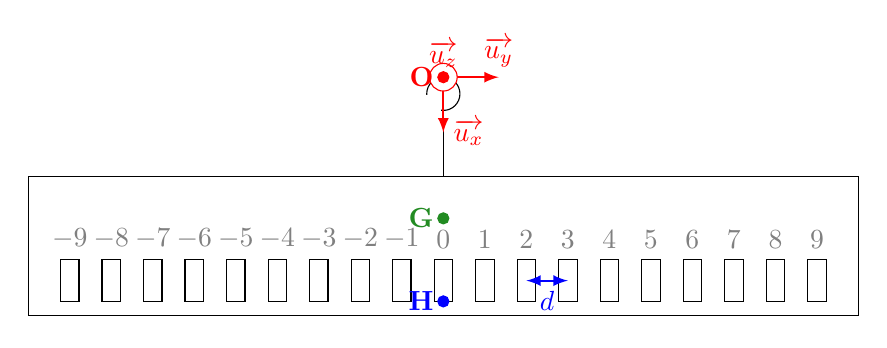
\begin{tikzpicture}
\draw (0pt,0pt) -- (0pt,50pt) ;
\node[shape = circle, minimum width=12pt, minimum height = 12pt, draw=black] at (0pt,55pt) {} ;
\node[shape = rectangle, minimum width=10pt, minimum height = 9pt, align=center, draw=white, fill=white] at (-6pt,50pt) {} ;
\node[shape = rectangle, minimum width=300pt, minimum height = 50pt, align=center, draw=black, fill=white] at (0pt,0pt) {} ;
\foreach \x in {-9,...,9} 
  {\node[shape = rectangle, minimum width=5pt, minimum height = 15pt, draw=black] at (\x * 15pt, -12.5pt) {} ;
   \node at (\x * 15pt,2.5pt) {\color{gray}$\x$} ;}
\draw[->, >=latex, thick, draw=red, fill=red] (0pt,61pt) -- (0pt,41pt) node[right] {\color{red} $\mathbf{\overrightarrow{u_x}}$};
\draw[->, >=latex, thick, draw=red, fill=red] (0pt,61pt) -- (20pt,61pt) node[above] {\color{red} $\mathbf{\overrightarrow{u_y}}$};
\filldraw [draw=red, fill=white] ((0pt,61pt) circle (5pt) node[above] {\color{red} $\mathbf{\overrightarrow{u_z}}$};
\filldraw [draw=red, fill=red] ((0pt,61pt) circle (2pt) node[left] {\color{red} $\mathbf{O}$};
\filldraw [draw=ForestGreen, fill=ForestGreen] (0pt,10pt) circle (2pt) node[left] {\color{ForestGreen} $\mathbf{G}$};
\filldraw [draw=blue, fill=blue] (0pt,-20pt) circle (2pt) node[left] {\color{blue} $\mathbf{H}$};
\draw[<->, >=latex, thick, draw=blue, fill=blue] (30pt,-12.5pt) -- node[below] {\color{blue} $d$} (45pt,-12.5pt);%30N
\end{tikzpicture}
\caption{A hanger.}
\label{hanger}
\end{figure}


\section{Description of forces}

Lets now, imagine $n$ objects attached to the hanger.
The hanger is consider immobile (it does not fall and does not move like a pendulum).
The $k$th object have a mass $m_k$ and is attached to the position $p_k$.
We name $A_k$ the point where the object is attached.
We will detail all the forces applied to the hanger (see figure \ref{forces}):
\begin{itemize}
\item Its weight $\overrightarrow{W}$, applied in its gravity center. This force is directed downwards.
\item The reaction of the hook $\overrightarrow{R}$, applied in the point $O$ and directed upwards.
\item The weight of the $k$th object $\overrightarrow{W_k}$ applied its forces on the hook in the point $\overrightarrow{A_k}$. This force is directed downwards.
\end{itemize}

\begin{figure}
\centering
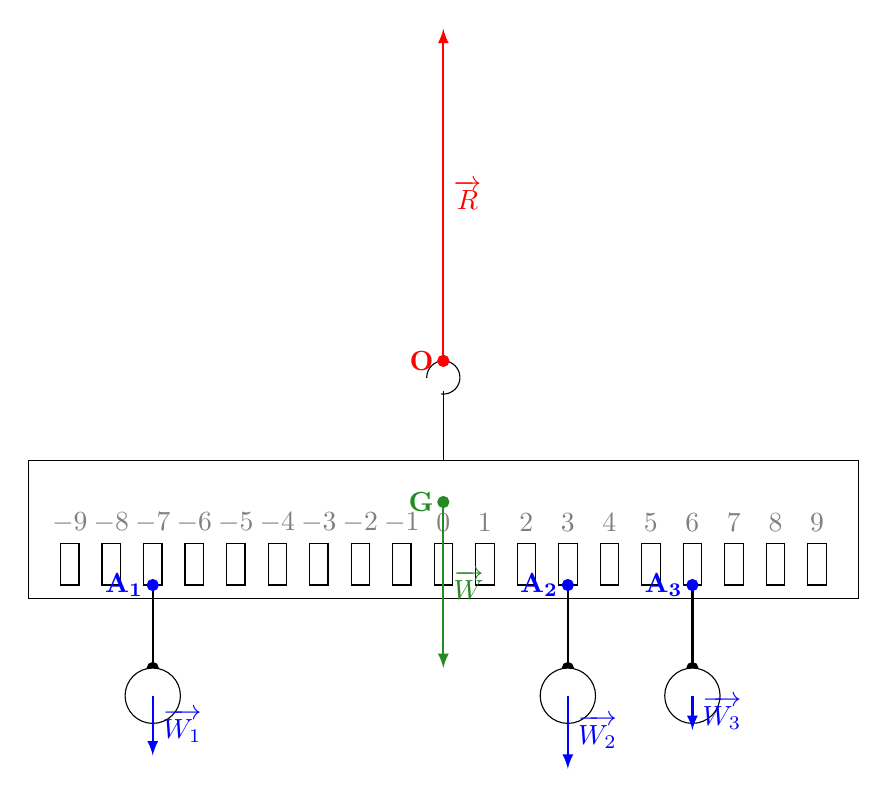
\begin{tikzpicture}
\draw (0pt,0pt) -- (0pt,50pt) ;
\node[shape = circle, minimum width=12pt, minimum height = 12pt, draw=black] at (0pt,55pt) {} ;
\node[shape = rectangle, minimum width=10pt, minimum height = 9pt, align=center, draw=white, fill=white] at (-6pt,50pt) {} ;
\node[shape = rectangle, minimum width=300pt, minimum height = 50pt, align=center, draw=black, fill=white] at (0pt,0pt) {} ;
\foreach \x in {-9,...,9} 
  {\node[shape = rectangle, minimum width=5pt, minimum height = 15pt, draw=black] at (\x * 15pt, -12.5pt) {} ;
   \node at (\x * 15pt,2.5pt) {\color{gray}$\x$} ;}
\draw[thick] (90pt,-20pt) -- (90pt,-50pt) ;
\filldraw ((90pt,-50pt) circle (2pt) {};
\node[shape = circle, minimum width=20pt, minimum height = 20pt, draw=black, fill=white] at (90pt,-60pt) {} ;
\draw[thick] (45pt,-20pt) -- (45pt,-50pt) ;
\filldraw ((45pt,-50pt) circle (2pt) {};
\node[shape = circle, minimum width=20pt, minimum height = 20pt, draw=black, fill=white] at (45pt,-60pt) {} ;
\draw[thick] (-105pt,-20pt) -- (-105pt,-50pt) ;
\filldraw ((-105pt,-50pt) circle (2pt) {};
\node[shape = circle, minimum width=20pt, minimum height = 20pt, draw=black, fill=white] at (-105pt,-60pt) {} ;
\filldraw [draw=red, fill=red] ((0pt,61pt) circle (2pt) node[left] {\color{red} $\mathbf{O}$};
\draw[->, >=latex, thick, draw=red, fill=red] (0pt,61pt) -- node[right] {\color{red} $\mathbf{\overrightarrow{R}}$} (0pt,181pt); %60N
\filldraw [draw=ForestGreen, fill=ForestGreen] (0pt,10pt) circle (2pt) node[left] {\color{ForestGreen} $\mathbf{G}$};
\draw[->, >=latex, thick, draw=ForestGreen, fill=ForestGreen] (0pt,10pt) -- node[right] {\color{ForestGreen} $\mathbf{\overrightarrow{W}}$} (0pt,-50pt);%30N
\filldraw [draw=blue, fill=blue] (-105pt,-20pt) circle (2pt) node[left] {\color{blue} $\mathbf{A_1}$};
\filldraw [draw=blue, fill=blue] (90pt,-20pt) circle (2pt) node[left] {\color{blue} $\mathbf{A_3}$};
\filldraw [draw=blue, fill=blue] (45pt,-20pt) circle (2pt) node[left] {\color{blue} $\mathbf{A_2}$};
\draw[->, >=latex, thick, draw=blue, fill=blue] (-105pt,-60pt) -- node[right] {\color{blue} $\mathbf{\overrightarrow{W_1}}$} (-105pt,-81.6pt);%10.8N
\draw[->, >=latex, thick, draw=blue, fill=blue] (90pt,-60pt) -- node[right] {\color{blue} $\mathbf{\overrightarrow{W_3}}$} (90pt,-72.4pt);%6.2N
\draw[->, >=latex, thick, draw=blue, fill=blue] (45pt,-60pt) -- node[right] {\color{blue} $\mathbf{\overrightarrow{W_2}}$} (45pt,-86.4pt);%13.2N

\end{tikzpicture}
\caption{A balanced hanger (force vector are at the scale) with three mass.}
\label{forces}
\end{figure}

The weight oh an object is proportional to its mass. So :
\begin{itemize}
\item $\overrightarrow{P} = m g \overrightarrow{u_x}$ with $g = 9,806 65 m \cdot s^{-2}$.
\item $\overrightarrow{P_k} = m_k g \overrightarrow{u_x}$
\end{itemize}

The hanger is immobile. So its forces nullify :

\begin{tabular}{rcl}
   $\overrightarrow{W} + \overrightarrow{R} +  \underset{k = 1}{\overset{n}{\sum}} \overrightarrow{W_k}$ & = & $\overrightarrow{0}$\\
   $ W \overrightarrow{u_x} - R \overrightarrow{u_x} + \underset{k = 1}{\overset{n}{\sum}} W_k \overrightarrow{u_x}$ & = & $\overrightarrow{0}$\\
   $R$ & = & $W + \underset{k = 1}{\overset{n}{\sum}} W_k$ \\
   $R$ & = & $g  (m + \underset{k = 1}{\overset{n}{\sum}} m_k)$ \\
\end{tabular}

So, we have the value of the reaction of the hook.

\section{Condition of a balanced hanger}

In this section, we will consider a perfectly balanced hanger.
We will search necessary condition of this state.

The only movement the hanger can do is a rotation around the placed i is attached. So a rotation with an axis in $O$.
But the hanger is balanced so it is immobile when it is in a horizontal position.
This means that the sum of torques of forces around $O$ is zero.

The formula of the momentum in $O$ of the force $\overrightarrow{F}$ applied in $P$ is : $\overrightarrow{M}_{\overrightarrow{F}/O } = \overrightarrow {OP} \wedge \overrightarrow{F}$.
So we will look at the torque of each forces applied on the hanger :
\begin{itemize}
\item \begin{tabular}{rcll}
$\overrightarrow{M}_{\overrightarrow{R}/O } $ & = & $\overrightarrow {OO} \wedge \overrightarrow{R}$ & \\
$\overrightarrow{M}_{\overrightarrow{R}/O } $ & = & $\overrightarrow{0}$ & because $\overrightarrow {OO} = \overrightarrow{0}$\\
\end{tabular}
\item \begin{tabular}{rcll}
$\overrightarrow{M}_{\overrightarrow{W}/O } $ & = & $\overrightarrow {OG} \wedge \overrightarrow{W}$ & \\
$\overrightarrow{M}_{\overrightarrow{R}/O } $ & = & $\overrightarrow{0}$ & because in the case of a balanced hanger, $\overrightarrow {OG}$ and $\overrightarrow {W}$ are colinear to $\overrightarrow{u_x}$\\
\end{tabular}
\item \begin{tabular}{rcll}
$\overrightarrow{M}_{\overrightarrow{W_k}/O } $ & = & $\overrightarrow {OA_k} \wedge \overrightarrow{W_k}$ & \\
$\overrightarrow{M}_{\overrightarrow{W_k}/O } $ & = & $(\overrightarrow {OH} + \overrightarrow {HA_k}) \wedge \overrightarrow{W_k}$ & \\
$\overrightarrow{M}_{\overrightarrow{W_k}/O } $ & = & $(\overrightarrow {OH} \wedge \overrightarrow{W_k}) + (\overrightarrow {HA_k} \wedge \overrightarrow{W_k})$ & \\
$\overrightarrow{M}_{\overrightarrow{W_k}/O } $ & = & $\overrightarrow {0} + (\overrightarrow {HA_k} \wedge \overrightarrow{W_k})$ & because $\overrightarrow {OH}$ and $\overrightarrow {W_k}$ are colinear to $\overrightarrow{u_x}$\\
$\overrightarrow{M}_{\overrightarrow{W_k}/O } $ & = & $(HA_k \overrightarrow {u_x}) \wedge (W_k \overrightarrow{u_y}$ & \\
$\overrightarrow{M}_{\overrightarrow{W_k}/O } $ & = & $HA_k . W_k \overrightarrow{u_z}$ & \\
$\overrightarrow{M}_{\overrightarrow{W_k}/O } $ & = & $p_k . d . m_k . g \overrightarrow{u_z}$ & \\
\end{tabular}
\end{itemize}

So we can now sum up all the torque and search the case in which this sum nulify :
\begin{tabular}{rcll}
$\overrightarrow{M}_{\overrightarrow{R}/O} + \overrightarrow{M}_{\overrightarrow{W}/O} + \underset{k = 1}{\overset{n}{\sum}} \overrightarrow{M}_{\overrightarrow{W_k}/O}$ & = & $\overrightarrow{0}$ & \\
$\overrightarrow{0} + \overrightarrow{0} + \underset{k = 1}{\overset{n}{\sum}} p_k . d . m_k . g \overrightarrow{u_z}$ & = & $\overrightarrow{0}$ & \\
$\underset{k = 1}{\overset{n}{\sum}} p_k . d . m_k . g $ & = & $0$ & \\
$\underset{k = 1}{\overset{n}{\sum}} p_k . m_k $ & = & $0$ & \\
\end{tabular}aa

So the hanger is balanced if and only if the object check the condition: 
\begin{center}
$\underset{k = 1}{\overset{n}{\sum}} p_k . m_k = 0$
\end{center}


\section{Summary}

The hanger is balanced if and only if, when you sum up the product of masses of the object by the number of their position, yon obtain zero.




\chapter{Activities}




\end{document}
